\documentclass[A4,10pt,twocolumn]{IEEEtran}
%
\usepackage{setspace}
\usepackage{gensymb}
\doublespacing
\singlespacing

%\usepackage{graphicx}
%\usepackage{amssymb}
%\usepackage{relsize}
\usepackage[cmex10]{amsmath}
%\usepackage{amsthm}
%\interdisplaylinepenalty=2500
%\savesymbol{iint}
%\usepackage{txfonts}
%\restoresymbol{TXF}{iint}
%\usepackage{wasysym}
\usepackage{amsthm}
%\usepackage{iithtlc}
\usepackage{mathrsfs}
\usepackage{txfonts}
\usepackage{stfloats}
\usepackage{bm}
\usepackage{cite}
\usepackage{cases}
\usepackage{subfig}
%\usepackage{xtab}
\usepackage{longtable}
\usepackage{multirow}
%\usepackage{algorithm}
%\usepackage{algpseudocode}
\usepackage{enumitem}
\usepackage{mathtools}
\usepackage{steinmetz}
\usepackage{tikz}
\usepackage{circuitikz}
\usepackage{verbatim}
\usepackage{tfrupee}
\usepackage[breaklinks=true]{hyperref}
%\usepackage{stmaryrd}
\usepackage{tkz-euclide} % loads  TikZ and tkz-base
%\usetkzobj{all}
\usetikzlibrary{calc,math}
\usepackage{listings}
    \usepackage{color}                                            %%
    \usepackage{array}                                            %%
    \usepackage{longtable}                                        %%
    \usepackage{calc}                                             %%
    \usepackage{multirow}                                         %%
    \usepackage{hhline}                                           %%
    \usepackage{ifthen}                                           %%
  %optionally (for landscape tables embedded in another document): %%
    \usepackage{lscape}     
\usepackage{multicol}
\usepackage{chngcntr}
%\usepackage{enumerate}

%\usepackage{wasysym}
%\newcounter{MYtempeqncnt}
\DeclareMathOperator*{\Res}{Res}
\renewcommand{\baselinestretch}{2}
\renewcommand\thesection{\arabic{section}}
\renewcommand\thesubsection{\thesection.\arabic{subsection}}
\renewcommand\thesubsubsection{\thesubsection.\arabic{subsubsection}}

\renewcommand\thesectiondis{\arabic{section}}
\renewcommand\thesubsectiondis{\thesectiondis.\arabic{subsection}}
\renewcommand\thesubsubsectiondis{\thesubsectiondis.\arabic{subsubsection}}

% correct bad hyphenation here
\hyphenation{op-tical net-works semi-conduc-tor}
\def\inputGnumericTable{}                                 %%

\lstset{
%language=C,
frame=single, 
breaklines=true,
columns=fullflexible
}
%\lstset{
%language=tex,
%frame=single, 
%breaklines=true
%}

\begin{document}
\newtheorem{theorem}{Theorem}[section]
\newtheorem{problem}{Problem}
\newtheorem{proposition}{Proposition}[section]
\newtheorem{lemma}{Lemma}[section]
\newtheorem{corollary}[theorem]{Corollary}
\newtheorem{example}{Example}[section]
\newtheorem{definition}[problem]{Definition}
%\newtheorem{thm}{Theorem}[section] 
%\newtheorem{defn}[thm]{Definition}
%\newtheorem{algorithm}{Algorithm}[section]
%\newtheorem{cor}{Corollary}
\newcommand{\BEQA}{\begin{eqnarray}}
\newcommand{\EEQA}{\end{eqnarray}}
\newcommand{\define}{\stackrel{\triangle}{=}}

\bibliographystyle{IEEEtran}
\bibliographystyle{ieeetr}
\providecommand{\mbf}{\mathbf}
\providecommand{\pr}[1]{\ensuremath{\Pr\left(#1\right)}}
\providecommand{\qfunc}[1]{\ensuremath{Q\left(#1\right)}}
\providecommand{\sbrak}[1]{\ensuremath{{}\left[#1\right]}}
\providecommand{\lsbrak}[1]{\ensuremath{{}\left[#1\right.}}
\providecommand{\rsbrak}[1]{\ensuremath{{}\left.#1\right]}}
\providecommand{\brak}[1]{\ensuremath{\left(#1\right)}}
\providecommand{\lbrak}[1]{\ensuremath{\left(#1\right.}}
\providecommand{\rbrak}[1]{\ensuremath{\left.#1\right)}}
\providecommand{\cbrak}[1]{\ensuremath{\left\{#1\right\}}}
\providecommand{\lcbrak}[1]{\ensuremath{\left\{#1\right.}}
\providecommand{\rcbrak}[1]{\ensuremath{\left.#1\right\}}}
\theoremstyle{remark}
\newtheorem{rem}{Remark}
\newcommand{\sgn}{\mathop{\mathrm{sgn}}}
\providecommand{\abs}[1]{\left\vert#1\right\vert}
\providecommand{\res}[1]{\Res\displaylimits_{#1}} 
\providecommand{\norm}[1]{\left\lVert#1\right\rVert}
%\providecommand{\norm}[1]{\lVert#1\rVert}
\providecommand{\mtx}[1]{\mathbf{#1}}
\providecommand{\mean}[1]{E\left[ #1 \right]}
\providecommand{\fourier}{\overset{\mathcal{F}}{ \rightleftharpoons}}
%\providecommand{\hilbert}{\overset{\mathcal{H}}{ \rightleftharpoons}}
\providecommand{\system}{\overset{\mathcal{H}}{ \longleftrightarrow}}
	%\newcommand{\solution}[2]{\textbf{Solution:}{#1}}
\newcommand{\solution}{\noindent \textbf{Solution: }}
\newcommand{\cosec}{\,\text{cosec}\,}
\providecommand{\dec}[2]{\ensuremath{\overset{#1}{\underset{#2}{\gtrless}}}}
\newcommand{\myvec}[1]{\ensuremath{\begin{pmatrix}#1\end{pmatrix}}}
\newcommand{\mydet}[1]{\ensuremath{\begin{vmatrix}#1\end{vmatrix}}}
%\numberwithin{equation}{section}
\numberwithin{equation}{subsection}
%\numberwithin{problem}{section}
%\numberwithin{definition}{section}
\makeatletter
\@addtoreset{figure}{problem}
\makeatother

\let\StandardTheFigure\thefigure
\let\vec\mathbf
%\renewcommand{\thefigure}{\theproblem.\arabic{figure}}
\renewcommand{\thefigure}{\theproblem}
%\setlist[enumerate,1]{before=\renewcommand\theequation{\theenumi.\arabic{equation}}
%\counterwithin{equation}{enumi}


%\renewcommand{\theequation}{\arabic{subsection}.\arabic{equation}}

\def\putbox#1#2#3{\makebox[0in][l]{\makebox[#1][l]{}\raisebox{\baselineskip}[0in][0in]{\raisebox{#2}[0in][0in]{#3}}}}
     \def\rightbox#1{\makebox[0in][r]{#1}}
     \def\centbox#1{\makebox[0in]{#1}}
     \def\topbox#1{\raisebox{-\baselineskip}[0in][0in]{#1}}
     \def\midbox#1{\raisebox{-0.5\baselineskip}[0in][0in]{#1}}

%\vspace{3cm}


\title{ASSIGNMENT 12.11.3.6}
\author{Shristy Sharma (EE22BNITS11001)}





% make the title area
\maketitle

\newpage

%\tableofcontents

\bigskip

\renewcommand{\thefigure}{\theenumi}
\renewcommand{\thetable}{\theenumi}
%\renewcommand{\theequation}{\theenumi}


%Download all python codes 
%
%\begin{lstlisting}
%svn co https://github.com/JayatiD93/trunk/My_solution_design/codes
%\end{lstlisting}

%Download all and latex-tikz codes from 
%
%\begin{lstlisting}
%svn co https://github.com/gadepall/school/trunk/ncert/geometry/figs
%\end{lstlisting}
%


\section{PROBLEM 1}
1. Find the equations of the planes that passes through three points.
\begin{enumerate}
\item $\vec{A}= \myvec{1\\1\\– 1}, \vec{B}=\myvec{6\\4\\– 5},\vec{C}= \myvec{– 4\\– 2\\3}$
\item $\vec{A}= \myvec{1\\1\\0}, \vec{B}= \myvec{1\\2\\1}, \vec{C}= \myvec{– 2\\2\\-1}$
\end{enumerate}
\section{Solution for 1}
Equation of plane is given by,
\begin{align}
\vec{n}^\top \vec{x} = c\\
\implies \myvec{1&1&-1\\6&4&-5\\-4&-2&3}^\top \vec{n}=\myvec{1\\1\\1}\\
\implies \myvec{1&6&-4\\ 1&4&-2\\ -1&-5&3} \vec{n} = \myvec{1\\1\\1}
\end{align}
the augmented matrix is given by,
\begin{align}
\myvec{1&6&-4&\vrule&1\\1&4&-2&\vrule&1\\-1&-5&3&\vrule&1}\\
\xleftrightarrow[R_3 \leftarrow R_3 + R_1]{R_2 \leftarrow R_2 - R_1}\\
\myvec{1&6&-4&\vrule&1\\1&-2&2&\vrule&0\\0&1&-1&\vrule&2}\\
\xleftrightarrow{R_2 \leftarrow \frac{-R_2}{2}} \\ 
\myvec{1&6&-4&\vrule&1\\0&1&-1&\vrule&0\\0&1&-1&\vrule&2}\\
\xleftrightarrow[{R_1 \leftarrow R_1 + 6R_2}] {R_3 \leftarrow R_3 - R_2}\\
\myvec{1&0&2&\vrule&1\\0&1&-1&\vrule&0\\0&0&0&\vrule&2}\\
\xleftrightarrow{R_3\leftarrow \frac{R_3}{2}} \\
\myvec{1&0&2&\vrule&1\\0&1&-1&\vrule&0\\0&0&0&\vrule&1}\\ 
\xleftrightarrow{R_1 \leftarrow R_1 - R_3}\\ 
\myvec{1&0&2&\vrule&0\\0&1&-1&\vrule&0\\0&0&0&\vrule&1} 
\end{align}
Since, all the elements in one of the row is 0. Therefore, there will be infinite solutions.
This signifies that the given points are collinear.
The direction vector of the line of collinear points will be,
\begin{align}
\vec{m}=\vec{B}-\vec{C} = \myvec{10\\6\\-8}
\end{align}
Since,the equation of a line is given by,
\begin{align}
\vec{x}=\vec{p}+  \lambda \vec{m}\\
\implies \vec{x}= \myvec{1\\1\\– 1} + \lambda \myvec{10\\6\\-8}
\end{align}
\begin{figure}[h!]
  \centering
   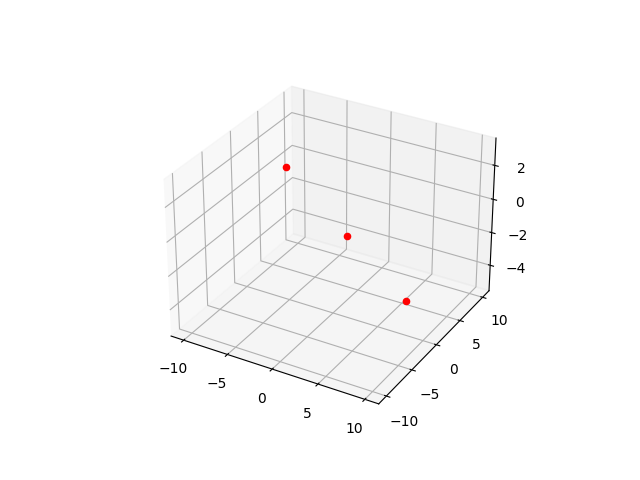
\includegraphics[width=\columnwidth]{figs/collinear_points.png}
    \caption{The figure shows that the given points are collinear}
     \label{fig:1}
     \end{figure}
\section{Solution for 2}
Equation of plane is given by,
\begin{align}
\vec{n}^\top \vec{x} = 1\\
\vec{x}^\top \vec{n}=1
\end{align}
Since, $\vec{A}, \vec{B}, \vec{C}$ satisfies this.
\begin{align}
\vec{A}^\top \vec{n}=1\\
%\implies \myvec{1\\1\\0} ^\top \vec{n}=1\\
  \vec{B}^\top \vec{n}=1\\
%\implies \myvec{1\\2\\1} ^\top \vec{n}=1\\
 \vec{C}^\top \vec{n}=1\\
%\implies \myvec{– 2\\2\\-1} ^\top \vec{n}=1\\
\implies \myvec{A^\top\\B^\top\\C^\top}  \vec{n} = 1\\
\implies \myvec{A&B&C}^\top\vec{n}=1\\
\implies \myvec{1&1&0 \\ 1&2&1 \\ -2&2&-1} ^\top \vec{n}=1\\
\implies \myvec{1&1&-2\\1&2&2\\0&1&-1}\vec{n}=1
\end{align}
the augmented matrix is given by,
\begin{align}
\myvec{1&1&-2&\vrule&1\\1&2&2&\vrule&1\\0&1&-1&\vrule&1}\\
\xleftrightarrow[R_3 \leftarrow R_3 - R_2]{R_2 \leftarrow R_2 - R_1}\\
\myvec{1&1&-2&\vrule&1\\0&1&4&\vrule&0\\0&0&-5&\vrule&1}
\end{align}
\begin{align}
\xleftrightarrow[R_1 \leftarrow 5R_1 - 2R_3]{R_2 \leftarrow 5R_2 + 4R_3}\\
\myvec{5&5&0&\vrule&3\\0&5&0&\vrule&4\\0&0&-5&\vrule&1}\\
\xleftrightarrow{R_1 \leftarrow R_1 - R_2}\\
\myvec{5&0&0&\vrule&-1\\0&5&0&\vrule&4\\0&0&-5&\vrule&1}\\
{R_1 \leftarrow \frac{R_1}{5}} ; {R_2 \leftarrow \frac{R_1}{5}}; {R_3 \leftarrow \frac{-R_3}{5}}\\
\myvec{1&0&0&\vrule&\frac{-1}{5}\\  \\ 0&1&0&\vrule&\frac{4}{5}\\ \\0&0&1&\vrule&\frac{-1}{5}}
\end{align}
Now, the equation of the plane will be,
\begin{align}
\myvec{\frac{-1}{5}\\ \\ \frac{4}{5}\\ \\ \frac{-1}{5}}^\top \vec{x} = 1
\end{align}
\begin{figure}[h!]
  \centering
   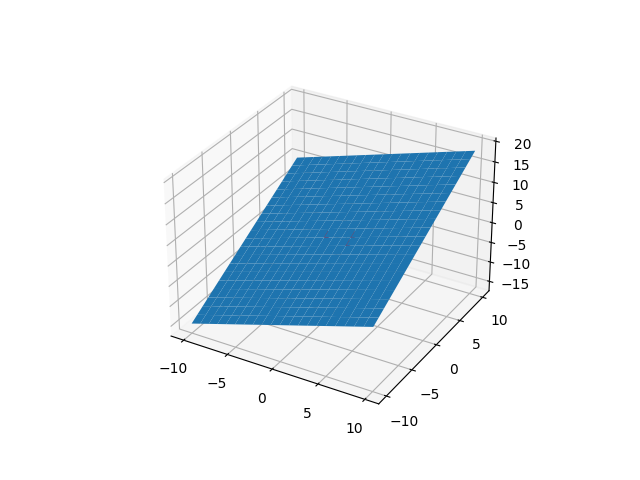
\includegraphics[width=\columnwidth]{figs/plane_b.png}
    \caption{Plane passing through the given points }
     \label{fig:2}
     \end{figure} 
\end{document}